%%%%%%%%%%%%%%%%%%%%%%%%%%%%%%%%%%%%%%%%%
% Journal Article
% LaTeX Template
% Version 1.4 (15/5/16)
%
% This template has been downloaded from:
% http://www.LaTeXTemplates.com
%
% Original author:
% Frits Wenneker (http://www.howtotex.com) with extensive modifications by
% Vel (vel@LaTeXTemplates.com)
%
% License:
% CC BY-NC-SA 3.0 (http://creativecommons.org/licenses/by-nc-sa/3.0/)
%
%%%%%%%%%%%%%%%%%%%%%%%%%%%%%%%%%%%%%%%%%

%----------------------------------------------------------------------------------------
%	PACKAGES AND OTHER DOCUMENT CONFIGURATIONS
%----------------------------------------------------------------------------------------

\documentclass[10pt]{article} % Single column

%\documentclass[twoside,twocolumn]{article} % Two column

\usepackage{blindtext} % Package to generate dummy text throughout this template 

\usepackage[sc]{mathpazo} % Use the Palatino font
\usepackage[T1]{fontenc} % Use 8-bit encoding that has 256 glyphs
\linespread{1.05} % Line spacing - Palatino needs more space between lines
\usepackage{microtype} % Slightly tweak font spacing for aesthetics

\usepackage[spanish]{babel} % Language hyphenation and typographical rules

\usepackage[hmarginratio=1:1,top=32mm,columnsep=20pt]{geometry} % Document margins
\usepackage[hang, small,labelfont=bf,up,textfont=it,up]{caption} % Custom captions under/above floats in tables or figures
\usepackage{booktabs} % Horizontal rules in tables

\usepackage{lettrine} % The lettrine is the first enlarged letter at the beginning of the text

\usepackage{enumitem} % Customized lists
\setlist[itemize]{noitemsep} % Make itemize lists more compact

\usepackage{abstract} % Allows abstract customization
\renewcommand{\abstractnamefont}{\normalfont\bfseries} % Set the "Abstract" text to bold
\renewcommand{\abstracttextfont}{\normalfont\small\itshape} % Set the abstract itself to small italic text

\usepackage{titlesec} % Allows customization of titles
\renewcommand\thesection{\Roman{section}} % Roman numerals for the sections
\renewcommand\thesubsection{\roman{subsection}} % roman numerals for subsections
\titleformat{\section}[block]{\large\scshape\centering}{\thesection.}{1em}{} % Change the look of the section titles
\titleformat{\subsection}[block]{\large}{\thesubsection.}{1em}{} % Change the look of the section titles

\usepackage{fancyhdr} % Headers and footers
\pagestyle{fancy} % All pages have headers and footers
\fancyhead{} % Blank out the default header
\fancyfoot{} % Blank out the default footer
\fancyhead[C]{Dise\~no y An\'alisis de Algoritmos. \textbf{Proyecto \# 1: La Pelota}} % Custom header text
\fancyfoot[RO,LE]{\thepage} % Custom footer text

\usepackage{titling} % Customizing the title section

\usepackage{hyperref} % For hyperlinks in the PDF

\usepackage{graphicx} % For images

\usepackage{pifont} % bullets

\usepackage{amsmath}



% Keywords command
\providecommand{\keywords}[1]
{
	\small	
	\vspace{0.5em}
	\noindent \textbf{\textit{Palabras clave --- }} #1
}


%----------------------------------------------------------------------------------------
%	TITLE SECTION
%----------------------------------------------------------------------------------------

\setlength{\droptitle}{-4\baselineskip} % Move the title up

\pretitle{\begin{center}\Huge\bfseries} % Article title formatting
	\posttitle{\end{center}} % Article title closing formatting
\title{\normalsize{Dise\~no y An\'alisis de Algoritmos }\\
	\Huge\bfseries Proyecto \# 1: La Pelota \\
} % Article title
\author{% 
	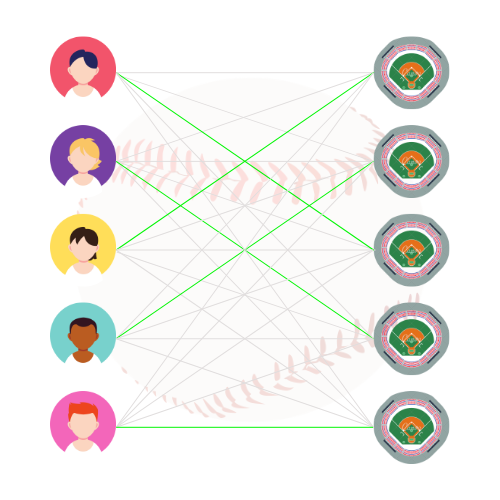
\includegraphics[width=15em]{logo.png}\\
	Laura Victoria Riera P\'erez\\
	Mari\'e del Valle Reyes \vspace{1em} \\
	\small Cuarto a\~no. Ciencias de la Computaci\'on. \\ % institution
	\small Facultad de Matem\'atica y Computaci\'on, Universidad de La Habana, Cuba \\ % institution
}
\date{\footnotesize \today } % Leave empty to omit a date


% Abstract configurations
\renewenvironment{abstract}
{\small
	\begin{center}
		\bfseries \abstractname\vspace{-.5em}\vspace{0pt}
	\end{center}
	\list{}{
		\setlength{\leftmargin}{1.5cm}%
		\setlength{\rightmargin}{\leftmargin}%
	}%
	\item\relax}
{\endlist}

\usepackage{amsthm}
\usepackage{amssymb}
\usepackage{todonotes} % \TODO
\usepackage{listings} % Code listings
\usepackage{xcolor}

\definecolor{backcolour}{rgb}{0.95,0.95,0.92}

\newcommand{\csl}[1]{\colorbox{backcolour}{\texttt{#1}}}

\newcommand{\imgcaption}[2]{\tiny \textbf{Figura #1.} #2.}

\newcommand{\mgc}[2][]{\colorbox{backcolour}{\texttt{\_\_#2\_\_#1}}}

\newcommand{\mgccapt}[1]{\texttt{\_\_#1\_\_}}

\newtheorem{thm}{Teorema}
\newtheorem{mydef}{Definici\'on}%[section]
\newtheorem{lem}{Lema}
\newtheorem{fig}{\scriptsize{Figura}}


\renewcommand{\qedsymbol}{\rule{0.7em}{0.7em}}

% Hyperlinks configurations
\hypersetup{
	colorlinks=true,
	linkcolor=black,
	filecolor=magenta,      
	urlcolor=cyan,
	pdftitle={Overleaf Example},
	pdfpagemode=FullScreen,
}

%----------------------------------------------------------------------------------------

\begin{document}
	% Print the title
	\maketitle
	
	%----------------------------------------------------------------------------------------
	%	ARTICLE CONTENTS
	%----------------------------------------------------------------------------------------
	
	\section{Repositorio del proyecto}
	
	\begin{center}
		\href{https://github.com/computer-science-crows/algorithms-design-and-analysis}{https://github.com/computer-science-crows/algorithms-design-and-analysis}
	\end{center}

	\section{Definici\'on inicial del problema} 
	
	Para un campeonato de pelota, el manager debe elegir de un conjunto de $ n $ personas, a su equipo de $ p $ jugadores, y a $ k $ espectadores especiales para que suban la moral del equipo.
	De cada persona $ i $, el manager conoce el valor que aporta a la moral del equipo $ a_i $ y el valor que aporta siendo situado en la posici\'on $ j $, $ s_{i,j} $. 
	Determine una alineación entre jugadores en el campo y espectadores de forma que el equipo tenga la mayor cantidad de valor acumulado posible.
	
	\section{Definici\'on en t\'erminos matem\'atico - computacionales}
	
	\subsection{Preliminares}
	
	\begin{mydef}
		Sea $ G= (V,E) $ un grafo. Se dice que $ G $ es bipartito si $ V(G) $ es la uni\'on de dos conjuntos independientes disjuntos. Si entre todo par de nodos de diferentes particiones existe una arista, se dice que es un grafo bipartito completo.
	\end{mydef}
	
	\begin{mydef}
		Un emparejamiento $ M $ es un conjunto de aristas en un grafo que son independientes, o sea, que no comparten v\'ertices.
	\end{mydef}

	\begin{mydef}
		Dado un emparejamiento $ M $ se dice que:
		\begin{itemize}
			\item Si la arista $ e = (v, w) \in M $, se dice que $ v $ y $ w $ son saturados por $ M $.
			\item Un conjunto de v\'ertices es saturado por $ M $ cuando $ M $ satura a todos los v\'ertices del conjunto.
			\item Se dice que $ M $ es perfecto si satura a $ V(G) $.
			\item $ M $ es m\'aximo cuando no existe $ M_{1} $ tal que $ |M_{1}| > |M| $.
		\end{itemize}
	\end{mydef}

	\begin{mydef}
		Sea $ G $ un grafo y $ M $ un emparejamiento del mismo. Un camino simple en $ G $ es $ M $-alternativo si sus aristas alternan entre pertenecer y no pertenecer a $ M $.
	\end{mydef}
	
	\begin{mydef}
		Sea $ G $ un grafo y $ M $ un emparejamiento del mismo. Un camino simple en $ G $ es $ M $-aumentativo si es $ M $-alternativo y sus extremos no son saturados por $ M $.
	\end{mydef}
	
	\begin{thm}
		Sea $ G $ un grafo y $ M $ un emparejamiento del mismo. M es maximal si y solo si no existen caminos $ M $-aumentativos.
	\end{thm}
%	\begin{proof}
%		($\Rightarrow$) Supongamos que M es maximal y existe alg\'un camino M-aumentativo. En el camino simple alternativo se pueden cambiar las aristas 
%	\end{proof}
	%\todo{Proof}
	
	\subsection{Problema de asignaci\'on}
	
	La entrada de nuestro problema es el n\'umero de personas $ n $, el n\'umero de posiciones a ser asignadas $ m = p + k $, donde $ p $ es la cantidad de posiciones dentro del equipo y $ k $ el n\'umero de asientos en el estadio a ser ocupados. Adem\'as, se recibe una lista $ a $ de valor aportado de cada persona por ser parte de la asignaci\'on, y una matriz $ s $ del valor aportado por cada persona en cada una de las posiciones. La salida del algoritmo debe ser la asignaci\'on de personas a posiciones que maximice el valor del equipo.
	
	Dado un grafo bipartito completo ponderado $G = (V,E)$, donde $V = L \cup R$. Se asume que los v\'ertices de los conjuntos $L$ y $R$ contienen $n$ v\'ertices cada uno, por tanto el grafo contiene $n^2$ aristas. Para todo $l \in L$ y $r \in R$, se denota el peso de la arista $(l,r)$ como $w(l,r)$, lo cual representa ganancia de emparejar el v\'ertice $l$ con el v\'ertice $r$. A encontrar un emparejamiento perfecto $M^*$ cuyas aristas tengan el peso m\'aximo total de todos los emparejamientos perfectos posibles se le llama \textit{problema de asignaci\'on}. Sea $w(M) = \sum_{(l,r) \in M} w(l,r)$ el peso total de las aristas en el emparejamiento $M$, se quiere encontrar el emparejamiento perfecto $M^*$ tal que,
	\[w(M*)=\text{max}\{w(M):M \text{ es un emparejamiento perfecto}\} .\]
	
	As\'i, nuestro problema puede ser modelado como un grafo bipartito completo ponderado $ G = (L \cup R, E) $ donde $ L $ representan las personas y $ R $ las posiciones en el estadio a ser asignadas; y donde el peso de cada arista $ e = (u, v) $ es $ w(e) = a[u] + s[u][v] $ .
	
	\section{L\'inea de pensamiento}
	
	Como primera soluci\'on al problema de asignaci\'on fue implementado un \textit{backtrack}. Esta es una soluci\'on correcta, ya que prueba todas las combinaciones y se queda con la que m\'as valor aporte, pero muy ineficiente, $ O(n!) $. En una computadora de 32GB de RAM, intel core i7-11na generaci\'on, se puede resolver para una cantidad m\'axima de personas y/o posiciones de 11. Dicha soluci\'on puede ser encontrada en \textit{src/solutions/backtrack\_solutions.py}.
	
	Se intent\'o resolver mediante un algoritmo \textit{greedy}, tomando por cada persona el m\'aximo del valor que puede aportar al equipo, y luego ir asignando de forma descendente a las posiciones. El problema de este enfoque est\'a en que cuando dos o m\'as personas aportan el mismo valor en una misma posici\'on se debe escoger aquel cuyo siguiente m\'aximo sea menor (pues de lo contrario en una pr\'oxima iteraci\'on se perder\'ia en valor en otra posici\'on). N\'otese que para el peor de los casos, cuando todos las personas aporten el mismo valor en todas las posiciones, esta soluci\'on es tan mala como backtrack.
	
	El pr\'oximo pensamiento fue resolverlo con \textit{programaci\'on din\'amica}. Para poder aplicar esta soluci\'on el problema debe cumplir con dos caracter\'isticas fundamentales: suproblemas solapados, es decir, que subproblemas iguales se repitan una y otra vez, por lo que se necesitar\'ia volver a calcular sus soluciones; y subestructura \'optima, lo cual significa que una soluci\'on \'optima para un subproblema forma parte de la soluci\'on \'optima del problema. Luego de graficar el backtrack y aplicar memorizaci\'on para varios casos se observ\'o que ninguno presentaba subproblemas solapados, por lo que la intuici\'on dice que probablemente no tenga.
	Adem\'as se cree que este problema no tiene subestructura \'optima (al menos para las formas de pensar y picar el mismo analizadas) dado que asignar las personas que m\'as valor den a un subconjunto de las posiciones no garantiza un \'optimo, puede ocurrir que esas personas aportaran m\'as en otras posiciones fuera del subconjunto. 
	
	Este problema puede ser modelado tambi\'en como un problema de optimizaci\'on lineal. Sea $ x_{i, j} $ una variable binaria que indica que se asign\'o la persona $ i $ a la posici\'on $ j $. Se quiere maximizar la suma de $ w(i, j) = a[i] + s[i, j] \forall i \in n, \forall j \in m $. Las restricciones a\~nadidas  garantizan que todos los v\'ertices tengan exactamente un vecino, y por tanto la soluci\'on hallada sea un emparejamiento perfecto. 
	
	\begin{equation} \left\{
	\begin{matrix}
		\max & \displaystyle z=\sum_{i}\sum_{j}x_{i,j}\cdot(s_{i,j} + a_{i}) \\
		\textrm{s.a.} & \sum_{j=1}^{m} x_{i, j} = 1 & \forall i \in n \\
		& \sum_{i=1}^{n} x_{i, j} = 1 & \forall j \in m \\ 
	\end{matrix} \right. 
	\end{equation} 

	Esta soluci\'on fue probada utilizando el algoritmo \textit{Simplex} implementado en la librer\'ia scipy y puede ser encontrada en \textit{src/solutions/simplex\_solution.py}. La complejidad temporal del simplex para el caso peor es O($ 2^{n} $), pero en general es bastante r\'apido.
	
	Investigando el estado del arte y siguiendo la idea de modelar el problems mediante grafos se decidi\'o implementar para su soluci\'on el algoritmo H\'ungaro descrito en \cite{introduction}, el cual es una especie de greedy y se ejecuta en tiempo polinomial, y es explicado en la pr\'oxima secci\'on. Dicha implementaci\'on est\'a en \textit{src/solutions/hungarian\_solution.py}.
	
	\section{Algoritmo H\'ungaro}

	El método Húngaro es un algoritmo de optimización-combinatoria que resuelve el problema de asignación en tiempo polinomial.
	
	En vez de trabajar con un grafo bipartito completo $G$, el algoritmo H\'ungaro trabaja con un subgrafo de $G$ llamado \textbf{subgrafo de igualdad}. El subgrafo de igualdad depende de asignar un atributo $h$ a cada v\'ertice. El atributo $h$ se llama \textbf{etiqueta} del v\'ertice. Se dice que $h$ es un \textbf{etiquetado de vértice factible} de $G$ si $l.h + r.h \geq w(l,r)$ para todo $l \in L$ y $r \in R$. Un etiquetado de v\'ertice factible siempre existe, como el \textbf{etiquetado de v\'ertice por defecto} dado por
	\begin{align}
		\label{eq:defecto}
		l.h &= \text{max} \{w(l,r):r \in R\} &\text{para todo } l \in R,\\
		r.h &= 0 &\text{para todo } r \in R 
	\end{align}
	
	Dado un etiquetado de v\'ertice factible $h$, el \textbf{subgrafo de igualdad} $G_h = (V, E_h)$ de $G$ consiste de los mismos v\'ertice de $G$ y el subconjunto de aristas $E_h = \{(l,r) \in E: l.h + r.h = w(l,r)\}$.
	
	El subgrafo de igualdad puede cambiar en el tiempo y tiene la propiedad que cualquier emparejamiento perfecto en el subgrafo de igualdad es tambi\'en una soluci\'on \'optima del problema de asignaci\'on como se demuestra en el siguiente teorema.
	\begin{thm} \cite{introduction}
		\label{thm: emparejamiento}
		Sea $G=(V,E)$, donde $V = L \cup R$, un grafo bipartito completo donde cada arista $(l,r) \in E$ tiene peso $w(l,r)$. Sea $h$ un etiquetado de v\'ertice factible de $G$ y $G_h$ el subgrafo de igualdad de $G$. Si $G_h$ contiene un emparejamiento perfecto $M^*$, entonce $M^*$ es una soluci\'on \'optima del problema de asignaci\'on $G$. 
		
	\end{thm}
	
	\begin{proof}
		Si $G_h$ tiene un emparejamiento perfecto $M^*$, entonces debido a que $G_h$ y $G$ tienen el mismo conjunto de v\'ertices, $M^*$ es tambi\'en un emparejamiento perfecto en $G$. Debido a que cada arista de $M^*$ pertenece a $G_h$ y cada v\'ertice tiene exactamente una arista incidente del emparejamiento perfecto, entonces se tiene
		
		\begin{align}
			w(M*) &= \sum_{(l,r) \in M*} w(l,r)\\
			&= \sum_{(l,r) \in M^*}(l.h + r.h) &\text{(porque todas las aristas de $M^*$ pertenecen a $G_h$)}\\
			&= \sum_{l \in L}l.h + \sum_{r \in R} r.h &\text{(porque $M^{*}$ es un emparejamiento perfecto)}\\
		\end{align} 
		
		Sea $M$ un emparejamiento perfecto cualquiera de $G$, se tiene
		
		\begin{align}
			w(M) &= \sum_{(l,r) \in M} w(l,r)\\
			&\leq \sum_{(l,r) \in M} (l.h + r.h) &\text{(porque $h$ es un etiquetado de v\'ertice factible)}\\
			&= \sum_{l \in L} l.h + \sum_{r \in R} r.h &\text{(porque $M$ es un emparejamiento perfecto)}
		\end{align}
		
		Entonces se tiene
		\begin{equation}
			w(M) \leq \sum_{l \in L} l.h + \sum_{r \in R} r.h = w(M^*),
		\end{equation}
		por tanto $M^*$ es un emparejamiento perfecto de m\'aximo costo en $G$.
	\end{proof}
	
	Entonces, el objetivo del algoritmo es encontrar un emparejamiento perfecto en un subgrafo de igualdad. 
	
	\subsection{Explicaci\'on del algoritmo}
	
	%El algoritmo H\'ungaro repetidamente modifica el emparejamiento y las etiquetas de v\'ertices en orden de alcanzar su objetivo.
	
	El algoritmo H\'ungaro empieza con un etiquetado de v\'ertice factible $h$ que es el de defecto \ref{eq:defecto} y cualquier emparejamiento $M$ en el subgrafo de igualdad $G_h$.  En la resoluci\'on de este problema se utiliz\'o un algoritmo de emparejamiento maximal greedy. Luego, el algoritmo repetidamente encuentra un \textbf{camino $M$-aumentativo} $P$ en $G_h$ utilizando una variante de B\'usqueda Primero a lo Ancho (\textit{en ingl\'es}, \textbf{BFS}). 
	
	El algoritmo BFS empieza la b\'usqueda desde todos los v\'ertices no saturados de $L$, los cuales al inicio se insertan en la cola $Q$. La condici\'on de parada es que se descubra alg\'un v\'ertice no saturado de $R$, ya que un camino $M$-aumentativo es aquel que empieza en un v\'ertice no saturado de $L$ y termina en un v\'ertice no saturado de $R$, tomando aristas no saturadas de $L$ a $R$ y aristas saturadas de $R$ a $L$. El resultado del algoritmo es un bosque primero a lo ancho $F = (V_f, E_f)$, donde cada v\'ertice no saturado de $L$ es ra\'iz de alg\'un \'arbol de $F$.
	
	
	Si la b\'usqueda de un camino $M$-aumentativo falla, se debe actualizar el etiquetado de v\'ertice factible para adicionar a $G_h$ al menos una arista nueva.
	
	Una vez encontrado un camino $M$-aumentativo, actualiza el emparejamiento para que este sea la diferencia sim\'etrica de $M$ y $P$, incrementando as\'i el tama\~no del emparejamiento.  Mientras haya alg\'un subgrafo de igualdad que contenga un camino $M$- aumentativo, el tama\~no del emparejamiento puede incrementar, hasta que un emparejamiento perfecto se logre.
	
	Existen casos en los que la cola $Q$ se vac\'ia sin que se halla llegado a encontrar un v\'ertice no saturado de $R$ que conforme un camino $M$-aumentativo. Cuando esto ocurre, el algoritmo H\'ungaro actualiza el etiquetado de v\'ertices factible $h$ de acuerdo al siguiente lemma.
	
	\begin{lem}
		\cite{introduction}
		Sea $h$ un etiquetado de v\'ertice factible en el grafo bipartito completo G con el grafo de igualdad $G_h$, y se $M$ un emparejamiento para $G_h$ y $F$ el bosque constru\'ido a partir de una B\'usqueda Primero a lo Ancho (en ingl\'es, BFS) sobre el subgrafo de igualdad $G_h$. Entonces, la etiqueta $h'$,
		\begin{equation}
			v.h' =  \left\{
			\begin{array}{ll}
				v.h-\delta & \text{si $v \in F_l$}, \\
				v.h+\delta & \text{si $v \in F_r$}, \\
				v.h & e.o.c \\
			\end{array} 
			\right.
		\end{equation}				
		donde 
		\begin{equation}
			\label{eqn:delta}
			\delta = min\{l.h + r.l - w(l,r): l\in F_l, r \in F_r\}
		\end{equation}
		con $F_l = L \cap V_f$ y $F_r = R \cap V_f$ son v\'ertices del bosque $F$ que pertenecen a $L$ y a $R$, respectivamente, es una etiqueta de v\'ertice factible para $G$ con las siguientes propiedades:
		\begin{enumerate}
			\item Si (u,v) es una arista de bosque F para $G_h$, entonces (u,v) $\in E_{h'}$.
			\item Si (l,r) pertenece al emparejamiento M para $G_h$, entonces (l,r) $\in E_{h'}$.
			\item Existen v\'ertices $l \in F_l$ y $r \in R - F_r$ tales que (l,r) $\notin E_h$, pero (l,r) $\in E_{h'}$.  
		\end{enumerate} 
	\end{lem}
	\begin{proof}
		Primero se demuestra que $h'$ es un etiquetado de v\'ertice factible para $G$. Debido a que $h$ es un etiquetado de v\'ertice factible, se tiene $l.h + r.h \geq w(l,r)$ para todo $l \in L$ y $r \in R$. Para que $h'$ no sea un etiquetado de v\'ertice factible, entonces se necesitar\'ia que $l.h' + r.h' < l.h + r.h$ para alg\'un $l \in L$ y $r \in R$. La \'unica forma en que esto pudiera ocurrir ser\'ia para alg\'un $l \in F_l$ y $r \in R-F_r$. En esta instancia, la cantidad de decrecimiento es igual a $\delta$, entonces $l.h' + r.h' = l.h - \delta + r.h$. Por ecuaci\'on \ref{eqn:delta}, se tiene que $l.h - \delta + r.h \geq w(l,r)$ para cualquier $l \in F_l$ y $r \in R - F_r$, por tanto $l.h' + r.h' \geq w(l,r)$. Para cualquier otra arista, se tiene $l.h' + r.h' \geq l.h + r.h \geq w(l,r)$. Por tanto, $h'$ es un etiquetado de v\'ertice factible.
		
		Ahora se mostrar\'a la veracidad de las propiedades:
		\begin{enumerate}
			\item Si $l \in F_l$ y $r \in F_r$, entonces se tiene $l.h' + r.h' = l.h + r,h$ debido a que $\delta$ se adiciona a la etiqueta de $l$ y se substrae de la etiqueta de $r$. entonces, si una arista pertenece a $F$ para el grafo $G_h$, tambi\'en pertenece a $G_{h'}$.
			\item Se afirma que para el momentp en que el algoritmo H\'ungaro computa el nuevo etiquetado de v\'ertice factible $h'$, para toda arista $(l,r) \in M$, se tiene que $l \in F_l$ si y solo s\'i $r \in F_r$. 
			
			Para demostrar por qu\'e, se considera el v\'ertice saturado $r$ y la arista $(l,r) \in M$. 
			
			Primero se supone que $r \in F_r$, entonces la b\'usqueda encuentra $r$ y lo pone en la cola. Cuando $r$ se remueve de la cola, $l$ es descubierto, entonces $l \in F_l$. 
			
			Luego se supone que $r \notin F_r$, por tanto $r$ no se ha descubierto. Se demostrar\'a que $l \notin F_l$. La \'unica arista en $G_h$ que entra $l$ es $(r,l)$, y dado que $r$ no se ha descubierto, la b\'usqueda no ha tomado esta arista; si $l \in F_l$, no es por la arista ($r,l$). La \'unica otra forma que un v\'ertice en $L$ puede estar en $F_l$ es si es ra\'iz de la b\'usqueda, pero solo v\'ertices no saturados de $L$ son ra\'ices y $l$ est\'a saturado. Por tanto, $l \notin F_l$ y la afirmaci\'on se cumple.
			
			Se conoce que para $l \in F_l$ y $r \in F_r$ se cumple $l.h' + r.h' = l.h + r.h$. En caso contrario, cuando $l \in L-F_l$ y $r \in R-F_r$, se tiene que $l.h' = l.h$ y $r.h'=r.h$, entonces $l.h' + r.h' = l.h + r.h$. Por tanto, si la arista $(l,r)$ est\'a en el emparejamiento $M$ para el grafo $G_h$, entonces $(l,r) \in E_{h'}$.
			\item Sea $(l,r)$ una arista que no pertenece a $E_h$, tal que $l \in F_l$, $r \in R-F_r$ y $\delta = l.h + r.h - w(l,r)$. Entonces, por definici\'on de $\delta$, existe al menos una de esas arista. Luego, se tiene 
			
			\begin{align*}
				l.h' + r.h' &= l.h - \delta + r.h\\
				&= l.h - (l.h + r.h -w(l,r)) + r.h\\
				&= w(l,r)			
			\end{align*}
			y por tanto $(l,r) \in E_{h'}$. 
			
			
		\end{enumerate}
		
	\end{proof}
	
	%	Es posible que una arista pertenezca a $E_h$ pero no a $E_{h'}$.\todo{demostrar esto ex 25.3-3}
	
	\subsection{Complejidad Temporal}
	
	La complejidad temporal del algoritmo H\'ungaro implementado es $O(n^4)$, donde $|V|=2n$ y $|E|=n^2$ en el grafo original $G$.
	
	\section{Generador de casos de prueba}
	
	En \textit{src/app/generator.py} fue implementado un generador, el cual recibe una cantidad $ s $ de muestras a producir, genera valores random con el formato de entrada de los algoritmos implementados, halla la soluci\'on \'optima con $ backtrack $ y las guarda en $ json/test\_cases.json $. Se generaron 3000 casos de prueba, con $ n $ m\'aximo igual a 11, dado que, como se mencion\'o anteriormente, es lo que puede ejecutar el $ backtrack $.
	
	\section{Tester}
	 En \textit{src/app/tester.py} fue implementado un tester, que recibe una funci\'on y prueba el desempe\~no de la misma en cuanto a si obtuvo la soluci\'on \'optima o no, y el tiempo que demor\'o en hacerlo, comparando con los casos de prueba obtenidos con el generador. Dichos resultados se muestran en consola de la siguiente forma:
	 	 \begin{center}
	 		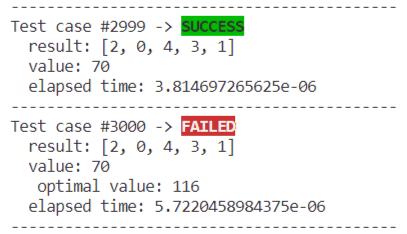
\includegraphics[width=7cm]{tester_sample.png}
	 		
	 		\tiny{\textbf{Figura 1.} Ejemplo de c\'omo se muestran los tests de una funci\'on en consola.} 
	 	\end{center}
 	 
 	 Adem\'as, estos resultados se guardan en un $ .json $ con el nombre de la funci\'on en la carpeta tests. Las soluciones implementadas fueron testeadas para todos los casos de prueba generados y pueden encontrarse en $ json/tests/simplex\_solution.json $ y $ json/tests/hungarian\_solution.json $
	
	\section{Comparaci\'on de soluciones implementadas}
	
	En los casos analizados, el \textit{backtrack} puede demorar desde menos de un segundo hasta casi dos minutos en ejecutarse. El \textit{simplex} demora para todos los casos menos de medio segundo, manteni\'endose para la mayor\'ia por debajo de los 0.2 segundos. Por \'ultimo el \textit{hungarian} implementado es el que mejores resultados muestra, tomando menos de 0.02 segundos para todos los casos, la d\'ecima parte de lo que demora el \textit{simplex}. A continuaci\'on se muestra una gr\'afica por cada algoritmo con el tiempo que demor\'o en cada uno de los 3000 tests. 
	\begin{center}
		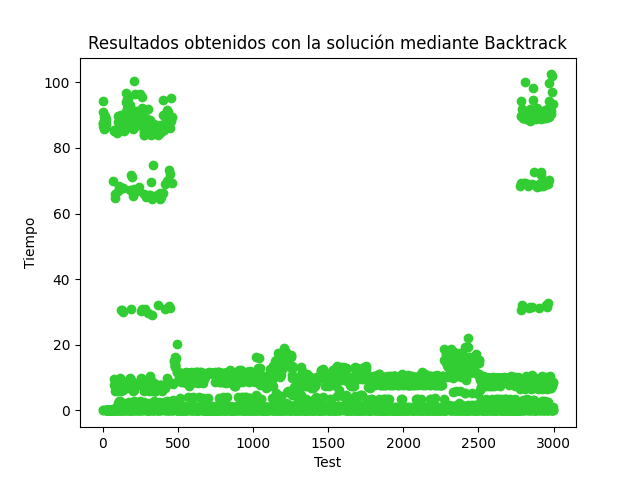
\includegraphics[width=7cm]{Backtrack_results.png}\\
		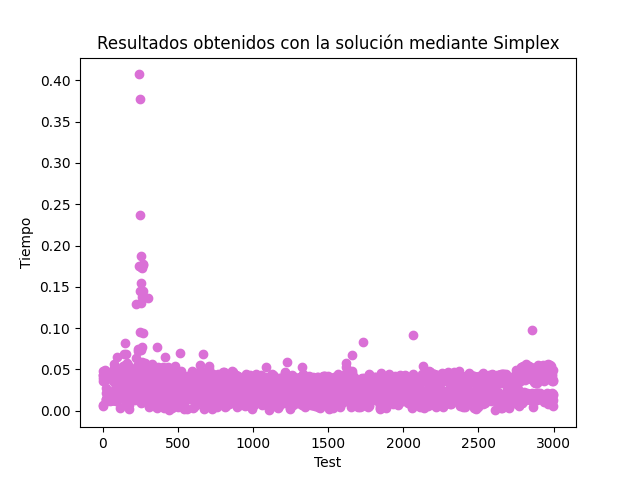
\includegraphics[width=7cm]{Simplex_results.png}
		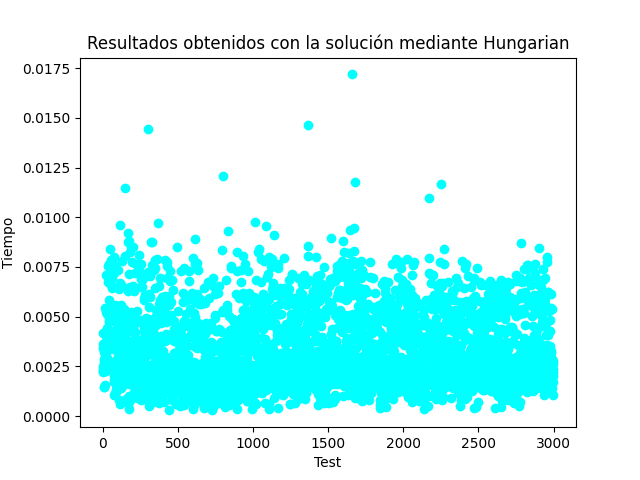
\includegraphics[width=7cm]{Hungarian_results.png}
	\end{center}  
	
	Adem\'as, en la siguiente gr\'afica se ofrece una comparaci\'on del tiempo promedio que le toma a cada algoritmo ejecutar los casos de prueba. 
	
	\begin{center}
		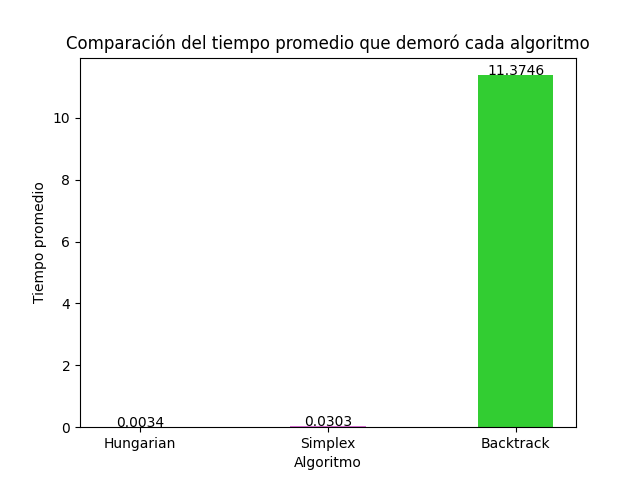
\includegraphics[width=7cm]{Bar_comparative_plot.png}
	\end{center}
	
	\begin{thebibliography}
		a
		\bibitem{introduction} Cormen, Thomas H. y otros. \emph{Introduction to Algorithms}. 
		The MIT Press.
		4ta Edici\'on.		
		Cambridge, Massachusetts.
		2022.
	\end{thebibliography}
\end{document}


